%! Author = gabriel
%! Date = 11/27/21

% Preamble
\documentclass[12pt,
    oneside,
    brazil,
    sumario=tradicional,
    article,
    a4paper
]{abntex2}

% Packages
\usepackage{setup/packages}


%! Author = gabriel
%! Date = 5/17/21

% --------------------------------------------
% Insira o nome do(s) autor(es).
% Caso seja mais de um, insira \and entre os
% nomes de cada um.
% --------------------------------------------
\author{Gabriel Medeiros Lopes Carneiro \\
        Emanuelle Maria Bottega Foscarini
}

% --------------------------------------------
% Insira o nome da universidade.
% --------------------------------------------
\university{Universidade Federal de Santa Catarina}

% --------------------------------------------
% Insira o nome do centro de ensino.
% --------------------------------------------
\educationcenter{Centro Tecnológico}

% --------------------------------------------
% Insira o nome do departamento de ensino.
% --------------------------------------------
\department{Departamento de Informática e Estatística}

% --------------------------------------------
% Insira o nome do curso ao qual pertence.
% --------------------------------------------
\course{Ciências da Computação}

% --------------------------------------------
% Afiliação do autor.
% -------------------------------------------- 
\affil{\printuniversity \par
        \printeducationcenter \par
        \printdepartment \par
        \printcourse}

%! Author = gabriel
%! Date = 5/17/21

% --------------------------------------------
% Insira o título do trabalho.
% --------------------------------------------
\title{Relatório}
% --------------------------------------------
% Caso o trablalho tenha subtítulo, descomente
% a linha abaixo.
% OBS.: NÃO APAGAR ":~" irá desconfigurar o arquivo.
% --------------------------------------------
\subtitle{:~Instalação e Execução do Nanvix}

% --------------------------------------------
% Insira o tipo de trabalho do documento.
% --------------------------------------------
\worktype{Tipo do trabalho}

% --------------------------------------------
% Insira o local de apresentação do documento.
% --------------------------------------------
\local{Florianópolis, SC}

% --------------------------------------------
% Define a data do documento. Por padrão mostra
% apenas o ano, caso queira a data completa,
% substitua por \today.
% --------------------------------------------
\date{\the\year}

% --------------------------------------------
% Caso o trabalho possua um orientador,
% comente a linha abaixo.
% --------------------------------------------
\orientador[Professor:]{Nome completo do professor}

% --------------------------------------------
% Caso o documento possua um orientador,
% descomente a linha abaixo.
% --------------------------------------------
%\orientador{Nome completo do orientador}

% --------------------------------------------
% Caso o documento possua um coorientador,
% descomente a linha abaixo.
% --------------------------------------------
%\coorientador{Nome completo do coorientador}

% --------------------------------------------
% Substituir '[mestre/doutor] em título obtido'
% pelo grau adequado.
% --------------------------------------------
%\formation{mestre/doutor em título obtido}

% --------------------------------------------
% Substituir nome do curso pelo nome do curso.
% --------------------------------------------
%\program{Programa de Pós-Graduação em nome do curso}

% --------------------------------------------
% Caso precise do preâmbulo do documento,
% descomente as linhas abaixo. Ele deve conter,
% o tipo do documento, o objetivo, o nome da
% instituição e a área de concentração.
% --------------------------------------------
%\preambulo{
%    \printworktype~ submetida ao
%    \printprogram~ da \printuniversity~
%    para a obtenção do título de \printformation.
%}

% --------------------------------------------
% Definição de cores de hyperlinks
% e formatações do pdf.
% --------------------------------------------
\hypersetup{
    colorlinks=true,
    linkcolor=black,
    filecolor=magenta,
    urlcolor=blue,
    citecolor=black,
    pdfauthor=\theauthor,
    pdftitle=\thetitle,
    bookmarksopen=true,
}
% Document
\begin{document}
    \printcoverufsc

    \section{Introdução}\label{sec:introducao}

    Esse relatório irá descrever os passos utilizados para a execução inicial do Nanvix, além dos problemas encontrados no caminho e resultado final da instalação.

    \section{Máquinas Usadas}\label{sec:máquinas-usadas}

    Todo o processo foi realizado em duas máquinas, abaixo segue uma descrição de seus hardwares e sistemas operacionais.

    \begin{enumerate}
        \item Máquina Ubuntu (Emanuelle)\label{maquina-ubuntu}
            \begin{itemize}
                \item Processador: IntelCore i7-4790S CPU @ 3.20GHz x 8.
                \item RAM: 16GB.
                \item Armazenamento: 240GB.
                \item Sistema Operacional: Ubuntu 20.04.3 LTS.
            \end{itemize}
        \item Máquina Mint (Gabriel)\label{maquina-mint}
            \begin{itemize}
                \item Processador: Ryzen 5 3600X 3.8GHz x 6.
                \item RAM: 16GB.
                \item Armazenamento: 240GB.
                \item Sistema Operacional: Linux Mint 20.2 Cinnamon Uma (baseado em Ubuntu 20.04 focal).
            \end{itemize}
    \end{enumerate}

    \section{Clonagem}\label{sec:clonagem}

    O primeiro passo foi a clonagem do repositório. A clonagem ocorreu sem mais problemas.
    
    \begin{figure}[!htb]
        \centering
        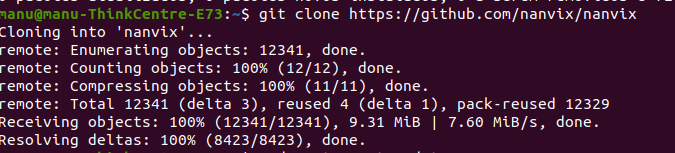
\includegraphics[scale=0.6]{cloning.png}
        \caption{Execução da clonagem do repositório.}
        \label{fig:cloning}
    \end{figure}
    
    \section{Ferramentas e Dependências}

    Depois da clonagem, foram instaladas as dependências listadas no guia básico (make, toolchain e bochs).
    A instalação das ferramentas foi concluída com sucesso em ambas as máquinas, apesar de demorar cerca de 30 minutos na máquina \ref{maquina-ubuntu} e menos de 10 minutos na máquina \ref{maquina-mint}.

    \section{Compilação}\label{sec:compilacao}

    Passando para a compilação do Nanvix, os dois comandos make foram executados sem erros em ambas as máquinas.
    Contudo, após rodar \textbf{make image} o arquivo \textit{nanvix.img} não foi encontrado, como mostra \autoref{fig:make}.

    \begin{figure}[!htb]
        \centering
        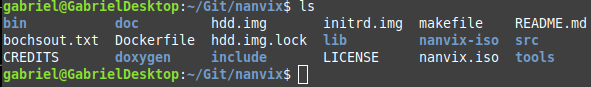
\includegraphics{make.png}
        \caption{Arquivos do nanvix após comandos make.}
        \label{fig:make}
    \end{figure}

    \section{Execução}\label{sec:execucao}

    Por último, realizamos a execução do Nanvix usando \textit{bash tools/run/run.sh} e ele abriu sem mais problemas, ilustrado na \autoref{fig:run-ubuntu} e na \autoref{fig:run-mint}.

    \begin{figure}[!htb]
        \centering
        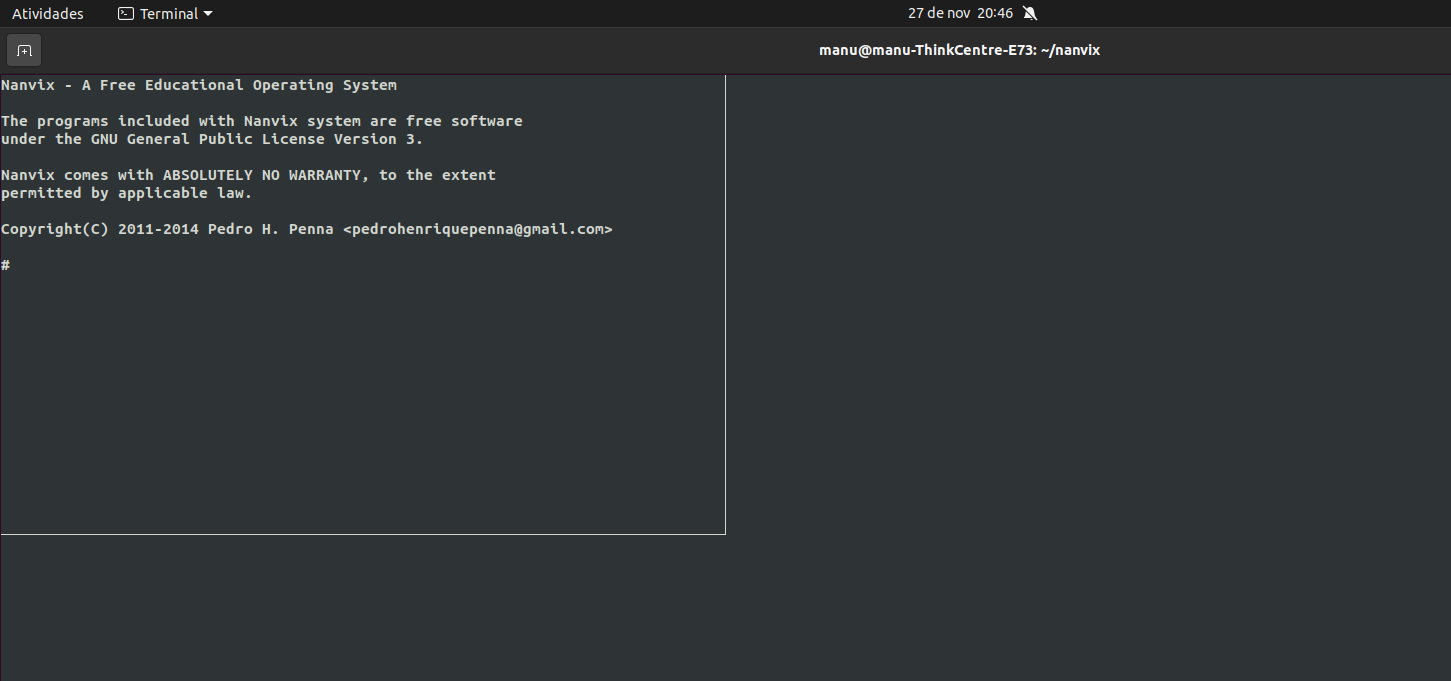
\includegraphics[scale=0.3]{run-ubuntu.png}
        \caption{Execução do Nanvix na máquina \ref{maquina-ubuntu}.}
        \label{fig:run-ubuntu}
    \end{figure}

    \begin{figure}[!htb]
        \centering
        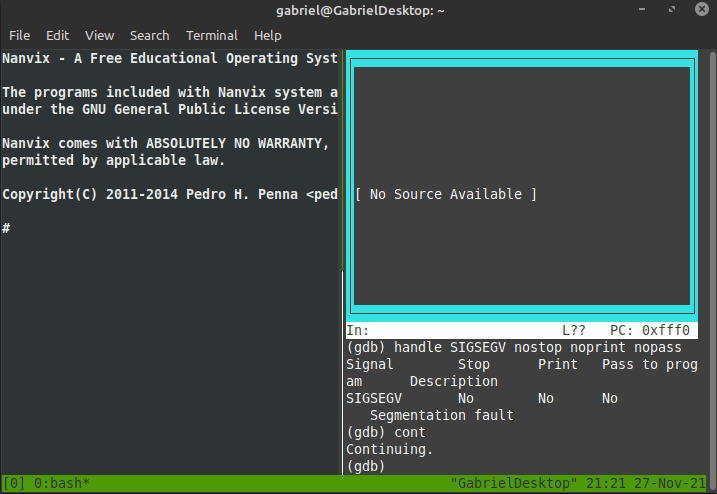
\includegraphics[scale=0.6]{run-mint.png}
        \caption{Execução do Nanvix na máquina \ref{maquina-mint}.}
        \label{fig:run-mint}
    \end{figure}

    \section{Conclusão}\label{conclusao}

    A instalação e execução do Nanvix foi simples e eficiente, sem apresentar grandes problemas durante a execução do relatório.

\end{document}